\documentclass[conference]{IEEEtran}
\IEEEoverridecommandlockouts
% The preceding line is only needed to identify funding in the first footnote. If that is unneeded, please comment it out.
\usepackage{cite}
\usepackage{amsmath,amssymb,amsfonts}
\usepackage{algorithmic}
\usepackage{graphicx}
\usepackage{textcomp}
\usepackage{xcolor}
\usepackage{tabularx}
\usepackage{multirow}
\usepackage{graphics} % for pdf, bitmapped graphics files
\usepackage{subfig}
\usepackage{subcaption}
\usepackage{hyperref}
\usepackage{academicons}
\usepackage{xcolor}
\usepackage{listings}
\usepackage{tabularx} % Asegúrate de incluir este paquete

\usepackage{tikz}
\usetikzlibrary{shapes.geometric, arrows}

\usetikzlibrary{shapes.geometric, arrows}

\tikzstyle{startstop} = [rectangle, rounded corners, minimum width=3cm, minimum height=1cm,text centered, draw=black, fill=red!30]
\tikzstyle{process} = [rectangle, minimum width=3cm, minimum height=1cm, text centered, draw=black, fill=blue!30]
\tikzstyle{arrow} = [thick,->,>=stealth]


\def\BibTeX{{\rm B\kern-.05em{\sc i\kern-.025em b}\kern-.08em
		T\kern-.1667em\lower.7ex\hbox{E}\kern-.125emX}}

% Color Enlace
\definecolor{colorEnlace}{RGB}{0, 0, 0}
\hypersetup{
	colorlinks=true,
	linkcolor=colorEnlace,
	citecolor=colorEnlace,
	urlcolor=colorEnlace,
	pdfauthor={Davis Bremdow Salazar Roa},
	pdftitle={Instrumentación Electrónica - ECG}
}
\definecolor{mybg}{rgb}{0.97,0.97,0.97}
\definecolor{mygray}{gray}{0.4}
\definecolor{mygreen}{rgb}{0,0.6,0}
\definecolor{myblue}{rgb}{0,0,0.8}
\definecolor{mypurple}{rgb}{0.58,0,0.82}
\definecolor{myred}{rgb}{0.7,0,0}

\lstdefinelanguage{MatlabEnhanced}{
	language=Matlab,
	morekeywords={[2]linspace,plot,title,xlabel,ylabel,legend,grid},
	morekeywords={[3]sin,cos,exp,log,sqrt},
	keywordstyle=\color{myblue}\bfseries,
	keywordstyle=[2]\color{mypurple},
	keywordstyle=[3]\color{myred},
	commentstyle=\color{mygreen}\itshape,
	stringstyle=\color{mygray},
	morecomment=[l]%
}

\lstset{
	language=MatlabEnhanced,
	backgroundcolor=\color{mybg},
	frame=single,
	basicstyle=\ttfamily\small,
	showstringspaces=false,
	numbers=none,              %
	xleftmargin=0pt,           %
	framexleftmargin=0pt,      
	framexrightmargin=0pt,
	framextopmargin=2pt,
	framexbottommargin=2pt,
	breaklines=true,
	tabsize=1,
}

% Control 
\usepackage{amsmath}
\begin{document}
	
	\title{Informe previo - Tensión de offset en amplificadores operacionales}
	\author{
		\makebox[\textwidth][c]{\large\textbf{Universidad Nacional de San Antonio Abad del Cusco}}\\
		\makebox[\textwidth][c]{\normalsize\textit{Escuela profesional de Ingeniería Electrónica}}\\
		\makebox[\textwidth][c]{\normalsize\textit{Asignatura: Instrumentación Electrónica}}\\
		\and
		\IEEEauthorblockN{Ing. Jose Luis Flores}
		\IEEEauthorblockA{Ingeniero Electrónico \\
			Cusco, Perú \\
			docente@unsaac.edu.pe}
		\and
		\IEEEauthorblockN{Davis Bremdow Salazar Roa - 200353}
		\IEEEauthorblockA{Estudiante de Ingeniería Electrónica \\
			Cusco, Perú \\
			200353@unsaac.edu.pe}
	}
	
	\maketitle
	\begin{abstract}
		
	\end{abstract}
	
	\begin{IEEEkeywords}
		
	\end{IEEEkeywords}
	
	%	Contenido del documento
	\section{Medición tensión eficaz (AC) y componente continua (DC)}
	
	Para la medición de estos parámetros se hizo uso del multímetro digital disponible en el laboratorio perteneciente al modelo 2110 de la marca Keithley, para ello se tomo como referencia la hoja de datos de este dispositivo y el esquema de conexión para la medición de voltaje como se muestra en la figura \ref{fig:configuracion-multimetro}
	
	\begin{figure}[h]
		\centering
		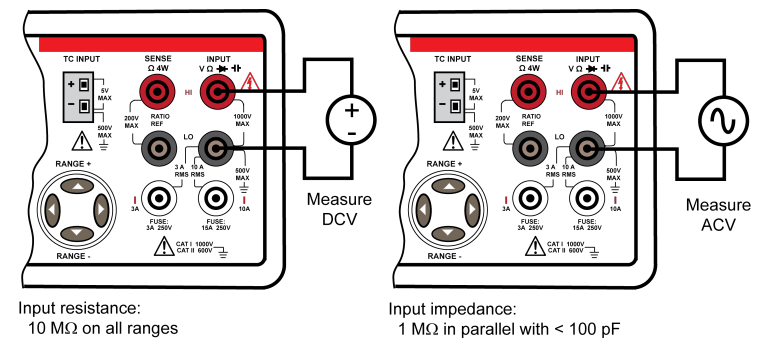
\includegraphics[width=0.5\textwidth]{media/configuracion-multimetro}
		\caption{Configuración Multimetro Keithley 2110}
		\label{fig:configuracion-multimetro}
	\end{figure}
	
	En la mediciones realizadas se obtuvieron valores determinados en la guía, siendo estos cercanos a 1.4140mV y 0v para las componentes AC y DC respectivamente.
	
	\section{Tensión continua y efecto del condensador $C_1$ y resistencia $R_1$}
	
	Al trabajarse con señales alternas durante el experimentación una medición DC en la resistencia $R_1$ tiene como resultado un valor de 0v, sin embargo al realizar esta misma medición para una configuración AC en el multímetro el capacitor $C_1$ y $R_1$ al tratarse de impedancia, esta actúa como un divisor de tensión w2 
	
	
	
	\bibliographystyle{IEEEtran}
	\bibliography{biblio}
\end{document}
o9